\documentclass[10pt, aspectratio=169]{beamer}

\usetheme[progressbar=frametitle, sectionpage=progressbar, subsectionpage=progressbar, numbering=fraction, block=fill]{metropolis}

\definecolor{mLightBrown}{HTML}{4D4D4D}
\definecolor{mMediumBrown}{HTML}{2C2C2A}
\definecolor{mDarkBrown}{HTML}{1A1A19}
\definecolor{mDarkTeal}{HTML}{0F6E56}
\definecolor{mDarkRed}{HTML}{B03A2E}
\setbeamercolor{normal text}{fg=mDarkBrown}
\setbeamercolor{alerted text}{fg=mDarkTeal}
\setbeamercolor{frametitle}{bg=mDarkBrown}
\setbeamercolor{progress bar}{fg=mDarkTeal, bg=mDarkTeal!20}
\definecolor{mPaleBg}{HTML}{F4F3EE}
\setbeamercolor{block title}{bg=mDarkBrown!10, fg=mDarkBrown}
\setbeamercolor{block body}{bg=mPaleBg, fg=mDarkBrown}
\newcommand{\hl}[1]{\textcolor{mDarkTeal}{#1}}

\usepackage{amsmath, amssymb, amsthm, mathtools}
\usepackage{cancel}\usepackage{bm}\usepackage{booktabs}\usepackage{array}
\usepackage{xcolor}\usepackage{colortbl}\usepackage{multirow}\usepackage{tikz}
\usetikzlibrary{positioning,arrows.meta,calc,fit,shapes.geometric,decorations.pathmorphing}

\newcommand{\paper}[1]{\textcolor{mLightBrown}{\small\textit{(#1)}}}

\newcommand{\qcur}{0}
\newcommand{\qnode}[4]{%
\ifnum#4=\qcur
 \node[draw=mDarkTeal, fill=mDarkTeal!12, thick, rounded corners=1pt, minimum width=3.0cm, minimum height=0.52cm, font=\tiny\bfseries, text=mDarkBrown] (#2) at (#1,0) {#3};%
\else
 \node[draw=mLightBrown!45, rounded corners=1pt, minimum width=3.0cm, minimum height=0.52cm, font=\tiny, text=mLightBrown] (#2) at (#1,0) {#3};%
\fi}
\newcommand{\qstrip}[1]{\renewcommand{\qcur}{#1}%
\begin{center}
\begin{tikzpicture}
\qnode{0}{q1}{Q1 Why a graph?}{1}
\qnode{3.7}{q2}{Q2 Independence?}{2}
\qnode{7.4}{q3}{Q3 Infer?}{3}
\qnode{11.1}{q4}{Q4 Decide?}{4}
\draw[-{Stealth}, mLightBrown!60] (q1.east) -- (q2.west);
\draw[-{Stealth}, mLightBrown!60] (q2.east) -- (q3.west);
\draw[-{Stealth}, mLightBrown!60] (q3.east) -- (q4.west);
\end{tikzpicture}\end{center}}

\title{Bayesian Networks}
\subtitle{A belief about many things is a graph}
\author{Jinkyoo Park}
\institute{KAIST}
\date{\textit{Lecture 3 --- Structured belief, and the first joining of belief to action}}

\begin{document}

\maketitle

%==========================================================
\section{The handoff --- belief over a whole system}
%==========================================================

\begin{frame}{Where we are --- from one unknown to many}
\vspace{2pt}
Lecture 2 carried a belief over \emph{one} parameter. Real systems have \alert{many interacting random variables}:
\begin{center}\footnotesize
a battery failure raises the chance of an electrical failure, which raises the chance of a communication loss \dots
\end{center}
\medskip

\pause
A joint distribution $p(x_1,\dots,x_n)$ over $n$ binary variables needs $2^n - 1$ numbers --- intractable to store, learn, or reason with. Belief over a system seems hopeless.
\medskip

\pause
\begin{center}\large
\alert{The escape is structure: a belief about many things is a graph.}
\end{center}
\medskip
\pause
Bayesian networks are where three threads meet: \textbf{probability} (the variables), \textbf{statistics} (the beliefs), and \textbf{graph theory} (the structure). The graph turns an exponential joint into a product of small, local pieces.
\end{frame}

\begin{frame}{The thesis --- structure tames the joint, and lets us act}
The fixed point of this lecture, in two parts:
\begin{center}\large
\alert{Conditional independence, drawn as a graph, makes belief over a system tractable ---}\\[2pt]
\alert{and adding decisions to that graph is the seed of all sequential decision-making.}
\end{center}
\medskip

\pause
The second half is the quiet bombshell of this lecture. So far the course has \emph{modeled} (Ch 1--2). Here, for the first time, a graphical model gains \alert{decision nodes and a utility node} --- belief, action, and value in one structure.
\medskip

\pause
That object --- the \emph{decision network} --- is a single-shot decision under uncertainty. Unroll it over time and it becomes the Markov Decision Process of Lecture 7. The lineage of dynamic decision-making starts here.
\end{frame}

\begin{frame}{The roadmap --- four questions}
\qstrip{0}
\medskip
\begin{itemize}\setlength\itemsep{3pt}
\item \textbf{Q1 --- Why represent a joint as a graph?} The factorization $p(x)=\prod_i p(x_i\mid \mathrm{pa}_i)$.
\item \textbf{Q2 --- What does the graph actually encode?} \alert{Conditional independence} --- and the savings it buys.
\item \textbf{Q3 --- How do we answer questions with it?} \alert{Inference}: marginalization and variable elimination.
\item \textbf{Q4 --- How do we add \emph{decisions}?} \alert{Decision networks} --- the seed of the MDP.
\end{itemize}
\end{frame}

%==========================================================
\section{Act 1 --- the joint as a graph}
%==========================================================

\begin{frame}{The factorization --- a joint, written locally}
\qstrip{1}
\medskip
A \alert{Bayesian network} is a distribution of the form
\[
p(x_1,\dots,x_n) = \prod_{i=1}^n p\big(x_i \mid \mathrm{pa}_{x_i}\big),
\]
a directed acyclic graph (DAG) where each node is a variable and edges point from parents to child.
\medskip
\begin{center}
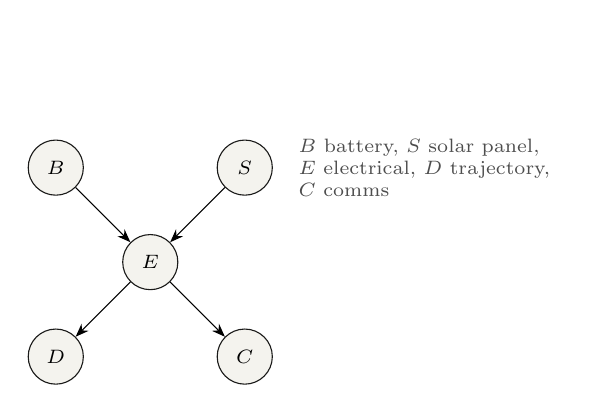
\begin{tikzpicture}[font=\scriptsize, node distance=10pt, every node/.style={draw=mDarkBrown, circle, minimum size=0.7cm, fill=mPaleBg}]
\node (B) at (0,1.2) {$B$};
\node (S) at (2.4,1.2) {$S$};
\node (E) at (1.2,0) {$E$};
\node (D) at (0,-1.2) {$D$};
\node (C) at (2.4,-1.2) {$C$};
\draw[-{Stealth}] (B)--(E); \draw[-{Stealth}] (S)--(E);
\draw[-{Stealth}] (E)--(D); \draw[-{Stealth}] (E)--(C);
\node[draw=none, fill=none, mLightBrown, right=4pt of S, align=left] {$B$ battery, $S$ solar panel,\\ $E$ electrical, $D$ trajectory,\\ $C$ comms};
\end{tikzpicture}
\end{center}
\medskip

\pause
Here $p(B,S,E,D,C) = p(B)\,p(S)\,p(E\mid B,S)\,p(D\mid E)\,p(C\mid E)$. Instead of one giant table, a handful of small \alert{local conditional tables} --- each node, given only its parents. The DAG \emph{is} the model.
\end{frame}

%==========================================================
\section{Act 2 --- what the graph encodes}
%==========================================================

\begin{frame}{Conditional independence --- the meaning of a missing edge}
\qstrip{2}
\medskip
Every distribution factorizes \emph{somehow} (the chain rule). What makes a BN powerful is that its graph asserts \alert{conditional independences}: a variable is independent of its non-descendants given its parents.
\medskip

\pause
\textbf{Why this is the whole point.}
\begin{itemize}\setlength\itemsep{1pt}
\item \textbf{Storage:} $2^n-1$ numbers collapse to a sum of small local tables --- exponential $\to$ linear in favorable structures.
\item \textbf{Learning:} far fewer parameters to estimate from data.
\item \textbf{Reasoning:} independence lets sums factor, making inference feasible (Act 3).
\end{itemize}
\medskip

\pause
\textbf{``Explaining away'' --- inference can be subtle.} Rain and sprinkler both wet the grass. Seeing wet grass raises belief in both; then learning the sprinkler was \emph{off} raises belief in rain. Two a-priori-independent causes become \alert{dependent once their common effect is observed}. The graph predicts exactly when such couplings arise.
\end{frame}

%==========================================================
\section{Act 3 --- reasoning with the network}
%==========================================================

\begin{frame}{Inference --- answering questions given evidence}
\qstrip{3}
\medskip
The core query: given evidence, what do we believe about a hidden variable? E.g.\ $P(B \mid d^1, c^1)$.
\medskip
\textbf{Exact inference} by marginalizing the joint:
\[
P(b^1\mid d^1,c^1) \;\propto\; \sum_{s}\sum_{e} P(b^1)P(s)P(e\mid b^1,s)P(d^1\mid e)P(c^1\mid e).
\]
\medskip

\pause
Done naively, the number of terms grows \alert{exponentially} in the hidden variables --- the curse returns.
\medskip

\pause
\textbf{Variable elimination} exploits the factorization: push each sum inward past factors that don't depend on it, eliminating one variable at a time into intermediate factors:
\[
P(b^1\mid d^1,c^1) \;\propto\; P(b^1)\sum_{e} P(d^1\mid e)P(c^1\mid e)\sum_{s} P(s)P(e\mid b^1,s).
\]
With a good elimination ordering the cost is often \emph{linear}; in the worst case still exponential (the ordering is a heuristic). Conditional independence is what makes the sums factor at all.
\end{frame}

%==========================================================
\section{Act 4 --- from belief to decision}
%==========================================================

\begin{frame}{Decision networks --- adding action and value to the graph}
\qstrip{4}
\medskip
\begin{center}\large
\alert{Bayesian Network $+$ decision node $+$ utility node $=$ Decision Network (influence diagram).}
\end{center}
\medskip
\begin{center}
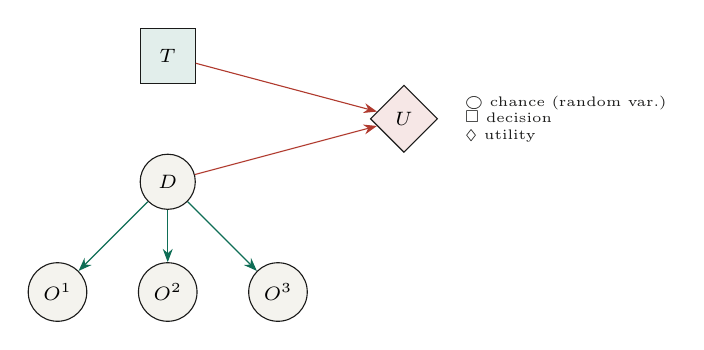
\begin{tikzpicture}[font=\scriptsize]
\node[draw=mDarkBrown, circle, fill=mPaleBg, minimum size=0.7cm] (D) at (0,0) {$D$};
\node[draw=mDarkBrown, rectangle, fill=mDarkTeal!12, minimum size=0.7cm] (T) at (0,1.6) {$T$};
\node[draw=mDarkBrown, diamond, fill=mDarkRed!12, minimum size=0.8cm] (U) at (3,0.8) {$U$};
\node[draw=mDarkBrown, circle, fill=mPaleBg, minimum size=0.55cm] (O1) at (-1.4,-1.4) {$O^1$};
\node[draw=mDarkBrown, circle, fill=mPaleBg, minimum size=0.55cm] (O2) at (0,-1.4) {$O^2$};
\node[draw=mDarkBrown, circle, fill=mPaleBg, minimum size=0.55cm] (O3) at (1.4,-1.4) {$O^3$};
\draw[-{Stealth}, mDarkTeal] (D)--(O1); \draw[-{Stealth}, mDarkTeal] (D)--(O2); \draw[-{Stealth}, mDarkTeal] (D)--(O3);
\draw[-{Stealth}, mDarkRed] (T)--(U); \draw[-{Stealth}, mDarkRed] (D)--(U);
\node[draw=none, right=6pt of U, align=left, font=\tiny]{\textcolor{mDarkBrown}{$\bigcirc$ chance (random var.)}\\ \textcolor{mDarkBrown}{$\square$ decision}\\ \textcolor{mDarkBrown}{$\Diamond$ utility}};
\end{tikzpicture}
\end{center}
\medskip

\pause
Three node types: \textbf{chance} (a random variable, as before), \textbf{decision} (an action we choose), \textbf{utility} (the value of an outcome). The optimal decision maximizes \alert{expected utility} over the posterior:
\[
d^* = \arg\max_{d}\; \mathbb{E}_{\text{posterior}}\big[\,U(d, \cdot)\,\big].
\]
\end{frame}

\begin{frame}{Why this is the hinge of the whole course}
A decision network is the first object in the course that contains all three ingredients of sequential decision-making at once:
\begin{center}\large
\textbf{belief} (chance nodes) $+$ \textbf{action} (decision node) $+$ \textbf{value} (utility node).
\end{center}
\medskip

\pause
\begin{block}{The seed}
\centering
A decision network is a \alert{single-shot} decision under uncertainty. \\
Unroll it over time --- state, action, reward, next state --- and it becomes the \alert{Markov Decision Process} of Lecture 7.
\end{block}
\medskip

\pause
So the line from here is direct: \emph{decision network} (one step) $\to$ \emph{MDP} (many steps, model given) $\to$ \emph{reinforcement learning} (many steps, model learned). Everything in Part IV is this one slide, extended through time and stripped of its model.
\end{frame}

%==========================================================
\section{Closing}
%==========================================================

\begin{frame}{Where we are --- belief structured, action attached}
\vspace{2pt}
\begin{center}\footnotesize\renewcommand{\arraystretch}{1.5}
\begin{tabular}{r|c|c}
 & \textbf{Model-based} & \textbf{Data-driven} \\
\hline
\textbf{Static, single}  & optimization \;{\scriptsize Lec.\ 1} & Bayesian stats \;{\scriptsize Lec.\ 2} $\to$ \cellcolor{mDarkTeal!15}\textbf{Bayesian networks} \;{\scriptsize Lec.\ 3 \checkmark}\\
\end{tabular}
\end{center}
\medskip

\pause
We can now represent belief over a whole system (a graph), reason within it (inference), and --- newly --- attach decisions and value to it. Two roads lead out:
\begin{itemize}\setlength\itemsep{1pt}
\item \textbf{Lecture 4:} put belief to work on an \alert{unknown function} --- a Gaussian process is a Bayesian network over a continuum of variables, and Bayesian optimization acts on it.
\item \textbf{Lecture 7:} unroll the decision network \alert{over time} into the MDP.
\end{itemize}
\end{frame}

\begin{frame}{Closing --- the one sentence}
\vfill
\begin{center}\large
A joint distribution over a system is unmanageable ---\\[8pt]
until conditional independence draws it as a graph,\\[4pt]
small local tables in place of one exponential one;\\[4pt]
and once we add a decision and a value to that graph,\\[4pt]
we have, in miniature, \alert{every decision problem still to come.}
\end{center}
\vfill
\pause
\footnotesize
Remember the decision network. It is the static, one-shot ancestor of the MDP, the dynamic program, and the reinforcement learner --- belief, action, and value, before time enters the picture.
\end{frame}

\begin{frame}[standout]
Questions?
\end{frame}

%==========================================================
\appendix
%==========================================================

\begin{frame}{Backup 1 --- variable elimination, step by step}
\footnotesize
Query $P(B\mid d^1,c^1)$ on the network $p(B,S,E,D,C)=p(B)p(S)p(E\mid B,S)p(D\mid E)p(C\mid E)$.
\medskip
\begin{enumerate}\setlength\itemsep{1pt}
\item \textbf{Insert evidence:} fix $D=d^1$, $C=c^1$, turning $p(D\mid E),p(C\mid E)$ into factors over $E$ alone.
\item \textbf{Eliminate $E$:} $\;T(B,S) = \sum_e p(e\mid B,S)\,p(d^1\mid e)\,p(c^1\mid e)$.
\item \textbf{Eliminate $S$:} $\;T'(B) = \sum_s p(s)\,T(B,s)$.
\item \textbf{Combine and normalize:} $\;P(B\mid d^1,c^1) \propto p(B)\,T'(B)$.
\end{enumerate}
\medskip
\textbf{Cost.} Each elimination creates an intermediate factor whose size is set by how many variables it couples --- the \emph{induced width} of the chosen ordering. A good ordering keeps factors small (often linear cost); a bad one creates large factors (exponential). Finding the optimal ordering is itself NP-hard, so heuristics are used --- the practical limit of exact inference, and the reason approximate (sampling) inference exists.
\end{frame}

\begin{frame}{Backup 2 --- the three canonical structures}
\footnotesize
Conditional independence in a BN is read off three building blocks (here $X \to Z \to Y$ etc.), governed by whether the middle node is observed:
\medskip
\begin{center}\scriptsize\renewcommand{\arraystretch}{1.35}
\begin{tabular}{l|l|l}
\textbf{Structure} & \textbf{Shape} & \textbf{$X \perp Y$ given $Z$?} \\
\hline
chain & $X \to Z \to Y$ & yes, if $Z$ observed (info flows through $Z$) \\
fork (common cause) & $X \leftarrow Z \to Y$ & yes, if $Z$ observed \\
collider (common effect) & $X \to Z \leftarrow Y$ & \alert{no} --- observing $Z$ \emph{creates} dependence \\
\end{tabular}
\end{center}
\medskip
The collider is ``explaining away'': $X$ and $Y$ are marginally independent but become dependent once their shared effect $Z$ is seen. Chaining these rules across a graph gives \alert{d-separation} --- the complete graphical test for whether any two sets of variables are conditionally independent given a third. It is how the DAG's edges translate, exactly, into independence assumptions.
\end{frame}

\begin{frame}{Backup 3 --- the maximum expected utility principle}
\footnotesize
A decision network computes the optimal decision by \alert{maximum expected utility} (MEU).
\medskip
\textbf{Setup.} Chance variables $X$ (with a BN), a decision $D$, a utility $U(D,X)$. Given evidence $e$, the posterior over the relevant chance variables is $p(x\mid d, e)$ (inference, Act 3).
\medskip
\textbf{Expected utility} of a decision $d$:
\[
\mathrm{EU}(d\mid e) = \sum_x p(x \mid d, e)\, U(d, x).
\]
\textbf{Optimal decision:} $\;d^* = \arg\max_d \mathrm{EU}(d\mid e)$, with value $\mathrm{MEU}(e) = \max_d \mathrm{EU}(d\mid e)$.
\medskip
\textbf{Connection forward.} Replace the single decision $D$ by a \emph{sequence} $d_0, d_1, \dots$, let each action move a state, and let utility accumulate as reward --- and MEU becomes the value function, $\arg\max_d \mathrm{EU}$ becomes the Bellman optimality operator. The MDP (Lecture 7) is this principle, iterated through time.
\end{frame}

\end{document}
